
\begin{figure}
    \centering
    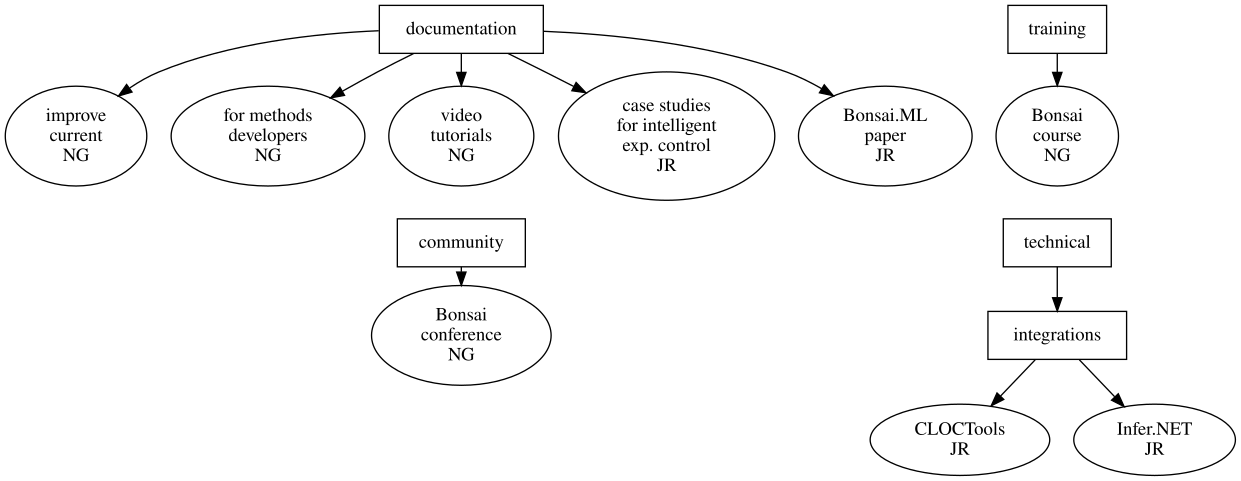
\includegraphics[width=6in]{activitiesGraphs/activities_larger.png}
    \caption{Proposed activities. See text for details.}
\end{figure}

\subsection*{Documentation}

We will improve the current Bonsai.ML
documentation\footnote[3]{\url{https://bonsai-rx.org/machinelearning/index.html}}
by:

\begin{enumerate}

    \item providing more detailed examples on the application of the
        already integrated ML methods to new types of behavioural and
        neural data.

    \item including video tutorials on the use of the Bonsai.ML
        package.

    \item adding documentation for methods developers, as the current one is
        targeted to Bonsai.ML users.

    \item creating case studies for intelligent experimental control in Bonsai,
        similar to the case studies for neural data analysis in
        Python\footnote[4]{\url{https://mark-kramer.github.io/Case-Studies-Python/intro.html}}.
        The aim of these case studies is to provide detailed ML training to
        Bonsai users.

    \item publishing a first Bonsai.ML paper describing its functionality.
        Publishing companion papers substantially increases the adoption of
        software packages \citep{lopesEtAl15,guilbeaultEtAl21}.

\end{enumerate}

\subsection*{Training}

Since 2017, NeuroGEARS Ltd (the non-profit organisation that is the main
contributor to the development of Bonsai) has organised at least two Bonsai
course per year at different universities, and some of them can be viewed
online\footnote[5]{\url{https://bonsai-rx.org/learn/}}. We will organise a new
Bonsai course with a module on Bonsai.ML.

\subsection*{Community}

Adding state-of-the-art ML methods and comprehensive documentation is critical.
However, from our previous experience with Bonsai, adoption will be low if we
do not demonstrate the impact of Bonsai.ML methods for solving important
neuroscience problems.
%
For this, we need to work closely with experimental neuroscientists to help
them solve relevant problems in intelligent experimental control.

\paragraph{Collaborations with experimental neuroscientists:} We will
collaborate with experimental neuroscientists at the Sainsbury Wellcome Centre,
and at the Institute for Behavioral Neuroscience (IBN) of University College London,
on the integration of machine learning functionality into their experiments.

\paragraph{Collaborations with methods developers;} Recently Prof.~Garrett
Stanley contacted us asking for assistance in integrating into Bonsai.ML
functionality for close-loop neural control that his laboratory had developed
in RTXI/C++\footnote[6]{\url{https://stanley.gatech.edu/}}. We will assist his
laboratory on this integration.

\subsection*{Governance}

We will create a Bonsai.ML governance structure comprising top-notch
neuroscientists that use Bonsai in their research and are heavily invested on
its future development.
%
This committee will advise us on building a long-term development roadmap for
Bonsai.ML.
